%!TEX root=paper.tex
\section{Evaluation}

The goal of our evaluation is to explore:

\begin{compactitem}

\item Whether, by varying $\lambda$, \textit{ShrinkNets} can efficiently
explore (in terms of number of training runs)  the spectrum of high-accuracy
models from small to large, on both CNNs and fully connected networks.  Our
results show that, for each network size, we obtain models that perform as well
or better than \textit{Static Networks}, trained via traditional hyperparameter
optimization.

\item Whether, because these  smaller networks are dense, they result in
improved inference times on both CPUs and GPUs.

\item Whether the ShrinkNets approach results in network architectures that are
substantially different than the best network architectures (in terms of
relative number of neurons per layered) identified in the literature.

\item \srm{something else?}

\end{compactitem}

\noindent\textbf{Implementation: }We implemented \textbf{switch Layers} and
the associated training procedure as a library in
pytorch~\cite{paszke2017automatic}. The layer can be freely mixed with other
popular layers such as convolutional layers, batchnorm layers, fully connected
layers, and used with all the traditional optimizers. We use our implementation
to evaluate ShrinkNets throughout the evaluation section.

\subsection{Can ShrinkNets achieve good accuracy?}
%\subsection{Performance vs. Traditional Methods}

To answer this question we compare ShrinkNets with a traditional network. In
both cases, we need to perform hyperparameter optimization to explore different
network architectures. We perform random search, which is an effective technique
for this purpose \cite{}. We evaluate ShrinkNets on two well-known datasets. One
for which it is not possible to explore the entire space of network
architectures (\texttt{CIFAR10}) and one for which it is possible to do so
(\texttt{COVERTYPE}).

\noindent\textbf{Setup: }
We assume no prior knowledge on the optimal batch size, learning rate, $\lambda$
or weight decay ($\lambda_2$). Instead, we trained a number of models, randomly
and independently selecting the values of these parameters from a range of
reasonable values (\gl{should we make them explicit ?} \srm{yes}).  
%We trained
%using our modified \texttt{PyTorch} \cite{paszke2017automatic} library that
%supports dynamically resized layers (our code is available at \srm{add
%anonymized link}). 
Training is done using gradient descent and the \textit{Adam}
optimizer \cite{DBLP:journals/corr/KingmaB14}. Specifically, we start with the
learning rate sampled randomly; for every $5$ epochs of non-improvement in
validation accuracy we divide the learning rate by $10$. We stop training after
$400$ epochs or when the learning rate is under $10^{-7}$, whichever comes
first.  \gl{Should I also give the details about the removal strategy we used
and the $\gamma$ and threshold I used ? because this is clearly getting boring}
\srm{probably not necessary} For each of the models we trained, we pick the
epoch with the best validation accuracy and report the corresponding testing
accuracy. Because of the nature of our method, it can happen that for networks
that are aggressively compressed, the best validation accuracy is obtained early
in  training, before the size has converged. To be sure that accuracy measured
corresponds to the final shape and not the starting shape, we only consider the
second half of the training when picking the best epoch. For each model, we also
measure the total size, in terms of number of floating point parameters,
excluding the \textit{Switch Layers} because as described in
\cref{neuron_killing}, these are eliminated after training.



%We evaluate ShrinkNets on two datasets:  \texttt{CIFAR10} and
%\texttt{COVERTYPE}. In this section, we report how we employed ShrinkNets on
%these datasets and compare our results to training without ShrinkNets.

\subsubsection{Large Network Setting: \texttt{CIFAR10}}

%\ra{this is related work}Previous research~\cite{Scardapane2017} that attempts
%to optimize network size during training focused on simple datasets and simple
%(i.e., fully connected) architectures. We believe that self-resizing network are
%most important for problems where the architecture involves many layers, such
%that that it is impractical to explore the space of all possible layer-size
%configurations.\ra{until here} 

\texttt{CIFAR10} is an image classification dataset containing $60000$ color
images $(3 \times 32 \times 32)$, belonging to $10$ different classes. We use it
with the \texttt{VGG16} network \cite{Srivastava2014}, which consists of
alternating convolutional layers and \textit{MaxPool} layers interleaved by
\textit{BatchNorm} \cite{DBLP:journals/corr/IoffeS15} and \textit{ReLU}
\cite{Nair2010}  layers.  The two last layers are fully connected layers
separated by a \textit{ReLU} activation function.

%\srm{keep this?} Although ShrinkNets supports larger networks and datasets as
%well (i.e., ImageNet \cite{ILSVRC15}),  the time required to such train models
%and get statistically significant result was prohibitive -- especially when
%comparing against classical hyperparameter search over network architecture.  

We applied ShrinkNets to the VGG16 network by adding \textit{Switch Layers}
after each \textit{BatchNorm} layer and each fully connected layer (except the
last).  Recall that ShrinkNets assume that the starting size of the network is
an upper bound on the optimal size. For this reason, we simply started with a
network with double the recommended size for each layer as an upper bound (this
is larger than what ImageNet, for example uses). Thus, for the classification
layers we use $5000$ neurons as a starting limit (ImageNet uses $4096$ \gl{This
is on the top of my head, need to be double checked}).

We compare against classical (\textit{Static}) networks. In such networks, the
number of parameters that control the size is large: 13 parameters for the
convolutional layers and $2$ for the fully connected layers. ShrinkNets
effectively fuse all these parameters in a single $\lambda$, but in conventional
architectures where all of these parameters are free, it is infeasible to obtain
a reasonable sample of a search space of this size. For this reason, we rely on
the conventional heuristic that the original VGG architecture (and many CNNs)
\gl{try to find the paper that introduces this heuristic} use, where
\srm{describe what the heuristic is -- doubling of neurons up to apoint?} For
\textit{Static Networks} we sample the size between $0.1$ and $2$ times the size
\srm{size of what?} optimized for ImageNet. \srm{Why are we using ImageNet and
not CIFAR10 as the comparison point?} We report the same numbers as we did for
\textit{ShrinkNets} and we compare the two distributions. \srm{I worry that
this method of selecting network sizes for Static will of course constrain it to
larger sizes and worse performance. What if we just randomly sample networks?
Would it look terrible?}

The results are shown in the top figure of \cref{figure_CIFAR10}, with blue dots
indicating ShrinkNet models and orange dots indicating static networks. For each
model, we plot its accuracy and model size. The lines show the Pareto frontier
of models in each of the two optimization settings. ShrinkNets explore the
trade-off between model size and accuracy more effectively. \srm{Would be good
to show Lambda values on the figure somehow.  } \srm{I thought we were going to
summarize with distributional plots instead of Pareto frontiers?} 
%\srm{Summarize
%more quantitatively -- best model performance, model performance drop off for a
%factor of 10 reduction in seize, etc. so that we can repeat a quantitative claim
%in the intro, i.e., ``Note that the best performing ShrinkNets models has 9x.x\%
%accuracy while the best static model has 9x.x\% accuracy, while the ShrinkNets
%model is x times smaller.  In addition, if we give up just 1\% error, ShrinkNets
%finds a model that is z times smaller.'' (If we do this, would be good to
%highlight these points in the figure somehow)}

Note that the best performing ShrinkNets models has \ra{xx} accuracy while the
best static model has \ra{xx} accuracy, while the ShrinkNets model is \ra{xx}
times smaller. In addition, if we give up just 1\% error, ShrinkNets finds a
model that is \ra{xx} times smaller. 

\subsubsection{Small Network Setting: \texttt{COVERTYPE}}

The \texttt{COVERTYPE} \cite{Blackard:1998:CNN:928509} dataset contains $581012$
descriptions of geographical area (elevation, inclination, etc...) and the goal
is to predict the type of forest growing in each area. We picked this dataset
for two reasons. First it is simple, such that we can reach good accuracy with
only a few fully-connected layers. This is important because we want to show
that \textit{ShrinkNets} find sizes as good as \textit{Static Networks}, even if
we are sampling the entire space of possible network sizes. Second, Scardapane
et al~\cite{Scardapane2017} perform their evaluation on this dataset, which
allows us to compare the results obtained by our method with the method in
~\cite{Scardapane2017}.

%The experimental setup on this dataset is similar to {\tt CIFAR10}. 
We compare ShrinkNets against the same architecture
used in \cite{Scardapane2017}, i.e., a three fully-connected layers network with no
\textit{Dropout} \cite{Srivastava2014} and no \textit{BatchNorm}. 
%\gl{Should we say
%here that we don't expect Dropout to work here ? I could write an entire
%paragraph about it if needed}. 
In this case, for the \textit{Static Networks}, we independently sample the
sizes of the three different layers to explore all possible architectures.

The results are shown in the top figure of \cref{figure_COVER}, with the two
optimization methods plotted as before. Here, {\it Static} method finds models
that perform well at a variety of sizes, because it is able to explore the
entire parameter space.  This is as expected;  the fact that ShrinkNets performs
as well as the Static indicates that ShrinkNets is doing an effective job of
exploring the parameter space using just the single $\lambda$ parameter.

Note that the best performing ShrinkNets models has \ra{xx} accuracy while the
best static model has \ra{xx} accuracy, while the ShrinkNets model is \ra{xx}
times smaller. In addition, if we give up just 1\% error, ShrinkNets finds a
model that is \ra{xx} times smaller. 

%\srm{Summarize more quantitatively -- best model performance, model performance
%drop off for a factor of 10 reduction in seize, etc. so that we can repeat a
%quantitative claim in the intro, i.e., ``Here, the best performing ShrinkNets
%models has 9x.x\% accuracy while the best static model has 9x.x\% accuracy,
%while the ShrinkNets model is x times smaller.  Further, note that ShrinkNets
%finds a model with 9x.x\% accuracy that is y times than the best performing
%model.  Also, as on CIFAR10, if we give up just 1\% error, ShrinkNets finds a
%model that is z times smaller.'' (If we do this, would be good to highlight
%these points in the figure somehow)}

\subsubsection{Summary}

We  demonstrated that it is possible to achieve networks with good accuracy
when using ShrinkNets both when the network space cannot be explored entirely
(\texttt{CIFAR10}) and when it can, e.g., \texttt{COVERTYPE}. The most important
result is not that ShrinkNets finds networks of good accuracy, but that those
networks are much smaller than those found by a static method. The impact of the
network size on inference time is the subject of our next evaluation goal.

%\srm{we may not need to keep this unless we can think of something more to say}
%
%The Pareto frontier in the two figures shows that 
%that \textit{ShrinkNets} is able find models that both as accurate and smaller than
%\textit{Static Networks}.
%
%when we sample the entire size space (in the \texttt{COVERTYPE} case),
%\textit{ShrinkNets} are better or equally as good as \textit{Static Networks}.
%This has two implications. First it reinforces our observation \srm{our observation?} in [ref] that
%showed that the models do not suffer from the non-convexity introduced by the
%multiplication by the \textit{Switch Layer}. Secondly it could let us conjecture
%that the parametrization from a $\lambda$ (real value) to the size of the
%size of the network (vector) close to optimal. Indeed, if it was
%not the case then eventually a randomly sampled size would have beaten
%\textit{ShrinkNets} models. \gl{Too strong ?} \srm{I think this is too strong -- we have no evidence this is true, do we?}
%

\subsection{Can ShrinkNets speed up inference?}

The previous experiment showed that ShrinkNets finds networks of similar or better accuracy
than static networks that are much smaller. We now explore if the reduction in size
translates into an improvement of the inference time.

%We showed in the previous experiments that the \textit{ShrinkNets} approach is
%able to find networks with accuracy equal to or better than \textit{Static
%Networks}. In this experiment we want to determine benefits of the smaller size
%we get.

As noted in the introduction, for some applications, compact models that offer fast inference times
are as important as absolute accuracy. 
%This observation motivates our 
% the experiment approach described in the previous section 
% and shown in the top of Figure~\ref{figure_CIFAR10} 
% and~\ref{figure_COVER}:
% for a  desired target accuracy, the Pareto optimal line shows the smallest
% network
% that satisfies achieves a given accuracy. 
In this section, we study the relationship between accuracy, network size and inference time.
To do this, we select the smallest model 
that achieves a given accuracy for the both ShrinkNets and Static approach.
For each model, we measure the time to run inference with the model.  
We then compute the ratio of the network size and inference time
between ShrinkNets and Static at each accuracy level, and plot them on the bottom of 
 Figure~\ref{figure_CIFAR10} 
 and~\ref{figure_COVER}.
We limit our plots to the models with $80-100\%$
accuracy range because those are the ones that we consider to be practically useful.

 The middle plot in each figure shows the ratio of model size between ShrinkNets and Static (values $>$1 mean ShrinkNets are smaller) at different accuracy levels.  These figures show that is that size improvements are are particularly significant
for  \texttt{CIFAR10}. In the range of accuracies we are interested in,
improvements in size go from 4x to 40x. On the \texttt{COVERTYPE} dataset,
 the compression ratio is always above 1 but it rarely exceeds 3x, except for
very high accuracies where \textit{ShrinkNets} finds excellent, small
solutions.  The fact that the  \texttt{COVERTYPE} networks are not dramatically 
smaller is expected:  as the distribution at the top of Figure~\ref{figure_COVER} shows,
the static method is able to explore most of the parameter search space, so finds a range
of models that perform well at different sizes.

For speedup, we experimented with both CPUs and GPUs, and with different batch sizes, where batch size indicates the number of inputs simultaneously fed to the model for inference.
For each data set/GPU/CPU combination, we show results with batch size 1, as well as with a batch size large enough to fully utilize the hardware on each dataset and hardware configuration.  For example, for {\tt CIFAR10} on CPU, a batch size of 64 fully utilizes the CPU, whereas a GPU can execute many more models in parallel, so we use a larger batch size of 1024.  For {\tt COVERTYPE}, because the model is so much smaller, larger batches are needed to fully utilize the hardware.
Note that when using a batch size of $1$ on GPU, we do not expect to (and do not) observe any improvement because inference times are very small (typically about 10 $\mu s$), such that setup time dominates overall runtime.  

 The bottom four graphs in each figure 
show the results.  Again, the {\tt CIFAR10} results show the benefit of the ShrinkNets approach
most dramatically.  On CPU, speedups range up to 6x depending on the batch size, with many models exceeding 3x speedup. In general, speedups are less than compression ratios, due to overheads in problem setup, invocation, and result generation  in Python/PyTorch.
  On GPU, the speedups are less substantial because the CUDA benchmarking utility that we use for evaluation can choose better algorithms for larger matrices which masks some of our benefit, although they are still often 1.5x--2x faster for large batch sizes.
The speedup results on {\tt COVERTYPE} are similar to those for network size:  because the networks are not much smaller, they are not much faster either.

A key takeaway of these speedup results is that, unlike local sparsity compression methods, our methods' improvement on size translates directly to higher throughput at inference time. \srm{Can we cite something showing that local sparsity does not improve performance even w/ small nets?}, at least for larger batches when hardware can be fully utilized.



%In situations in which inference is already fast (\texttt{COVERTYPE}
%with a batch size of $1$ and \texttt{CIFAR10} with a batch size of $1$ on GPU),
%improvements are dominated by noise. However, on machine learning frameworks
%more focused on latency it should be possible to measure them.


% \begin{figure}
% \begin{center}
% 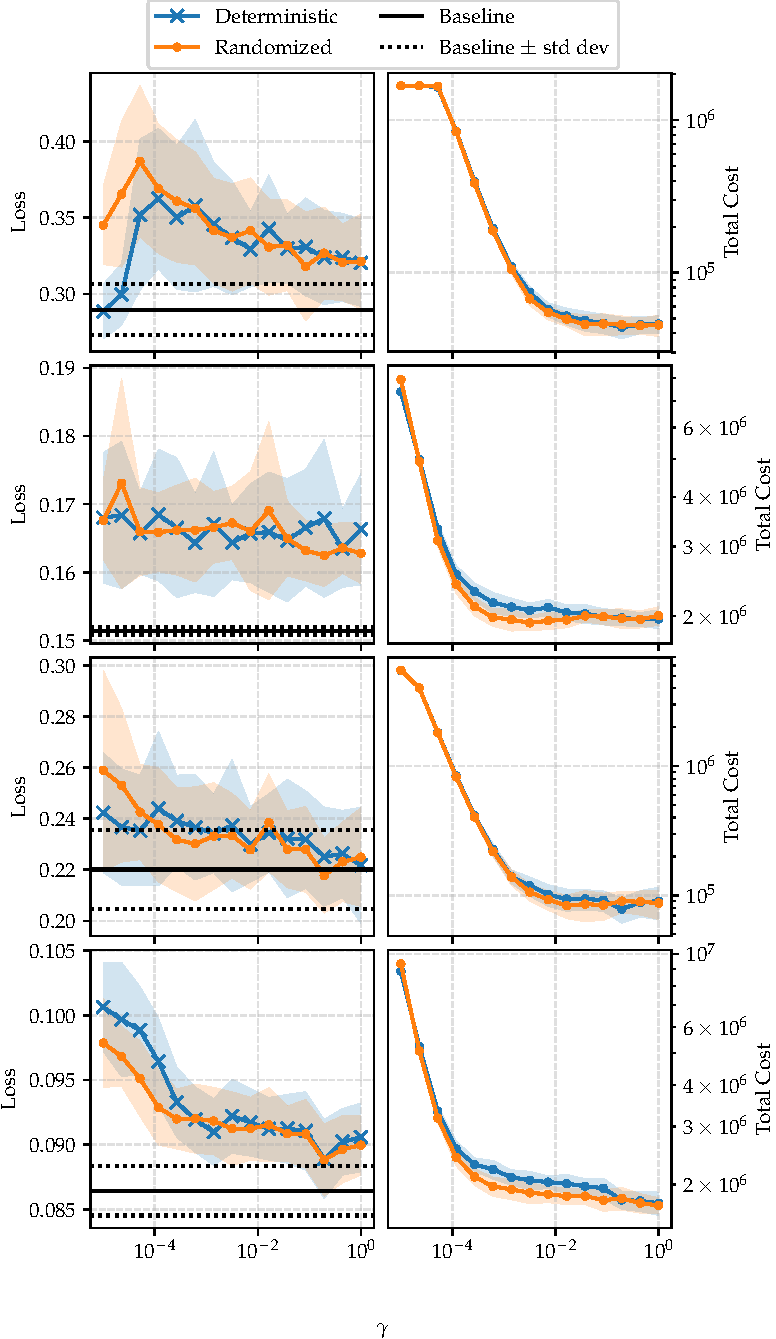
\includegraphics[width=\columnwidth]{neuron_removal}
% \vspace*{-5mm}
% \caption{\label{neuron_removal_figure}Effect of dynamic neuron removal for different $\gamma$. First column is the difference in the final loss in function of the removal factor. We plot theoretical baseline as a reference. Right column is a proxy of the total cost for training the model (i.e. the sum of input neurons at each epoch). Each row is a dataset/$\lambda$ combination. From top to bottom we have: \texttt{scm1d}/$0.1$, \texttt{oes97}/$0.1$}
% 
% \end{center}
% \vspace*{-4mm}
% \end{figure}

\begin{figure*}[t]\centering
\begin{minipage}{2.7in}
\begin{center}
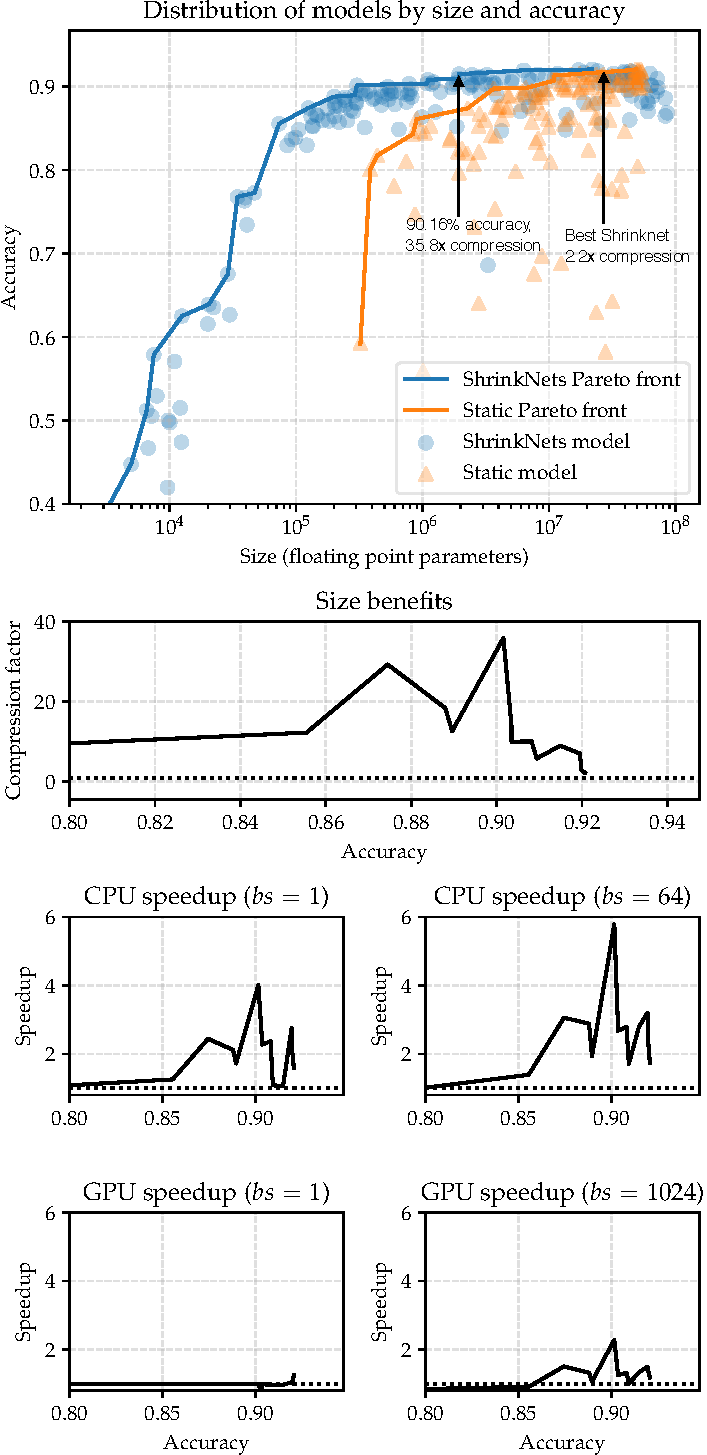
\includegraphics[width=\columnwidth]{CIFAR10_VGG_summary}
\vspace*{-5mm}
\caption{\label{figure_CIFAR10} Summary of the result of random
search over the hyper-parameters the \texttt{CIFAR10} dataset}
\end{center}
\vspace*{-4mm}
\end{minipage}
\begin{minipage}{2.7in}
\begin{center}
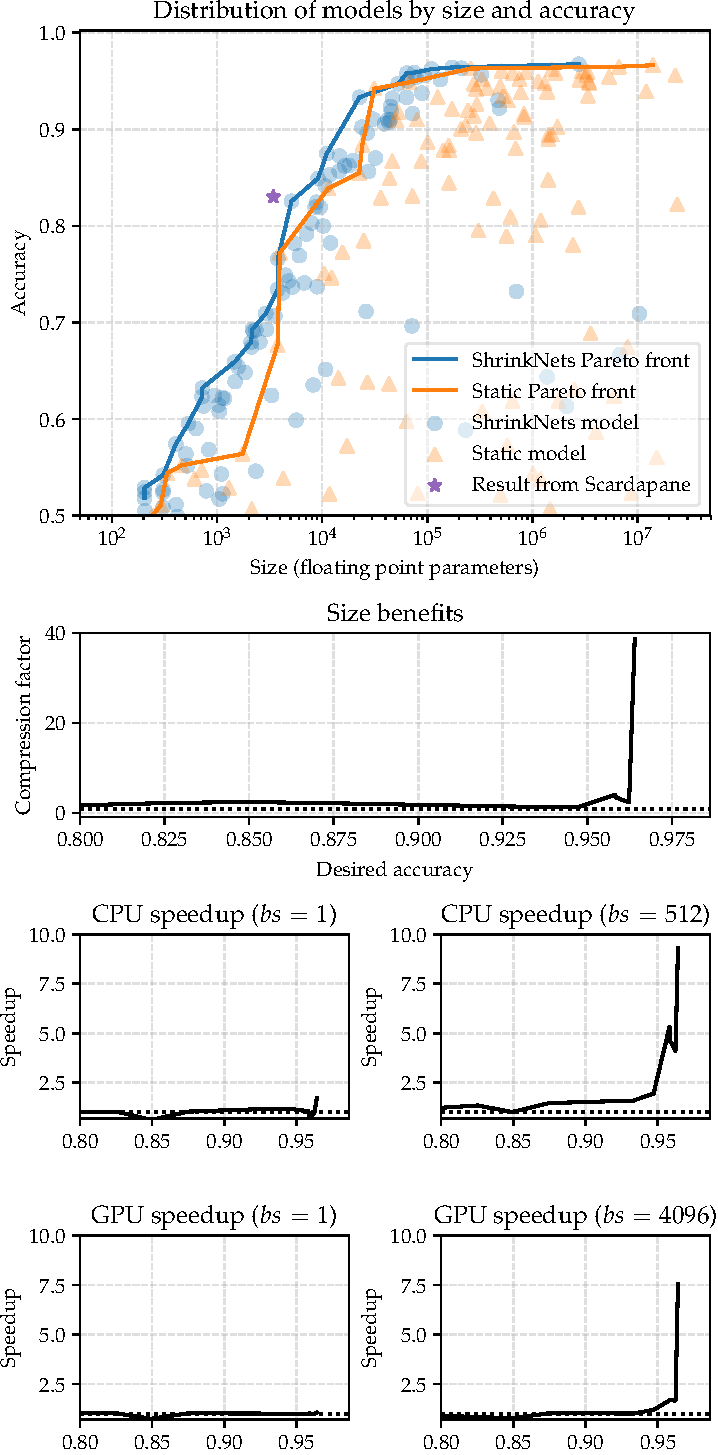
\includegraphics[width=\columnwidth]{COVER_FC_summary}
\vspace*{-5mm}
\caption{\label{figure_COVER} Summary of the result of random
search over the hyper-parameters the \texttt{COVERTYPE} dataset
\srm{label the x axes on the bottom plots; change ``Desired accuracy`` ``Accuracy''}
}
\end{center}
\vspace*{-4mm}
\end{minipage}
\end{figure*}

\ra{checkpoint}

\subsection{Architectures obtained after convergence}

\begin{figure}[htb]
\begin{center}
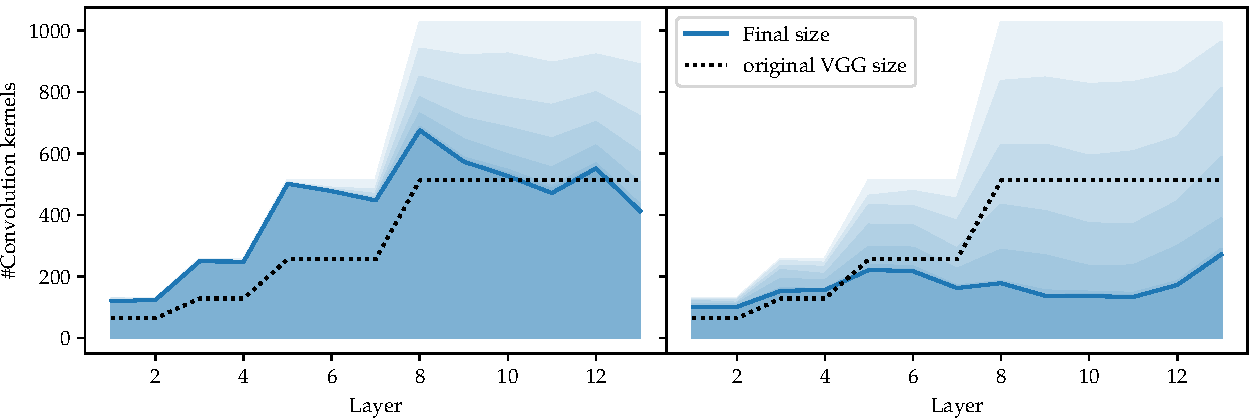
\includegraphics[width=.7\columnwidth]{size_evolution}
\vspace*{-5mm} 
\caption{ Evolution of the size of
  each layer over time (lighter: beginning, darker: end). On top a very large
  network performing $92.07\%$, at the bottom a simpler model with $90.5\%$
  accuracy. 
} 
\label{fig:network_size_evolution}
\end{center}
\vspace*{-4mm}
\end{figure}

\ra{the following is interesting, but how is it related to the above?}
ShrinkNets effectively explores the frontier of model size and accuracy. For a
given target accuracy, the size needed is significantly smaller than when we use the
\srm{name it} heuristic commonly used to size convolutional neural networks.
This suggests that this conventional heuristic may not in fact be optimal,
especially when looking for smaller models.  Empirically we observed this to
often be the case.  For example, during our experimentations on the
\texttt{MNIST} \cite{Lecun1998} and \texttt{FashionMNIST} \cite{Xiao2017}
datasets (not reported here due to space constraints), we observed that even
though these datasets have the same number of classes, input features, and
output distributions, for a fixed $\lambda$ \textit{ShrinkNets} converged to
considerably bigger networks in the case of \texttt{FashionMNIST}. This evidence
shows that optimal architecture not only depends on the output distribution or
shape of the data but actually reflects the dataset.  This makes sense, as
\texttt{MNIST} is a much easier problem than \texttt{FashionMNIST}.

To illustrate this point on a larger dataset, we show two examples of
architectures learned by \textit{ShrinkNets} in
Figure~\ref{fig:network_size_evolution}.  The top plot shows the model with the
best test accuracy, with \srm{identical performance to the best static
network?}; the bottom shows a network that slightly under-performs the best in
terms of accuracy but is significantly smaller that the best equivalent
\textit{Static Network} \srm{how much smaller?}.  In the plot, the dashed line
shows the number of neurons in each layer of the original VGG net, and the
shaded regions show the size of the ShrinkNet as it converges (with the darkest
region representing the fully converged network).  Observe that the final
network that is trained looks quite different in the two cases, with the optimal
performing network appearing similar to the original VGG net, whereas the
shrunken network allocates many fewer neurons to the middle layers, and then
additional neurons to the final fewer layers.


